\begin{lstlisting}[language=Python]
\end{lstlisting}

\hypertarget{amk-methods}{%
\section{Methods}\label{amk-methods}}

The practical implementation of what is described in this section is available as a Python package called Koala (Kitaev On Amorphous LAttices)~\autocite{hodsonKoalaKitaevAmorphous2022}. All results and figures were generated with Koala.

If we only care about the value of \(E_{u,0}\), it is possible to skip forming the fermionic operators. The eigenvalues obtained directly from diagonalising \(J^{\alpha} u_{ij}\) come in \(\pm \epsilon_m\) pairs. We can take half the absolute value of the whole set to recover \(\sum_m \epsilon_m\) easily.

\hypertarget{voronisation}{%
\subsection{Voronisation}\label{voronisation}}

To study the properties of the amorphous Kitaev model, we need to sample from the space of possible trivalent graphs.

A simple method is to use a Voronoi partition of the torus~\autocite{mitchellAmorphousTopologicalInsulators2018,marsalTopologicalWeaireThorpeModels2020,florescu_designer_2009}. We start by sampling \emph{seed points} uniformly (or otherwise) on the torus. Then, we compute the partition of the torus into regions closest (with a Euclidean metric) to each seed point. The straight lines (if the torus is flattened out) at the borders of these regions become the edges of the new lattice. The points where they intersect become the vertices.

The graph generated by a Voronoi partition of a two dimensional surface is always planar. This means that no edges cross each other when the graph is embedded into the plane. It is also trivalent in that every vertex is connected to exactly three edges \textbf{cite}.

Ideally, we would sample uniformly from the space of possible trivalent graphs. Indeed, there has been some work on how to do this using a Markov Chain Monte Carlo approach~\autocite{alyamiUniformSamplingDirected2016}. However, it does not guarantee that the resulting graph is planar, which we must ensure so that the edges can be 3-coloured.

In practice, we use a standard algorithm~\autocite{barberQuickhullAlgorithmConvex1996} from Scipy~\autocite{virtanenSciPyFundamentalAlgorithms2020} which computes the Voronoi partition of the plane. To compute the Voronoi partition of the torus, we take the seed points and replicate them into a repeating grid. This will be either 3x3 or, for very small numbers of seed points, 5x5. Then, we identify edges in the output to construct a lattice on the torus.

\hypertarget{fig:lattice_construction_animated}{%
\begin{figure}
\centering
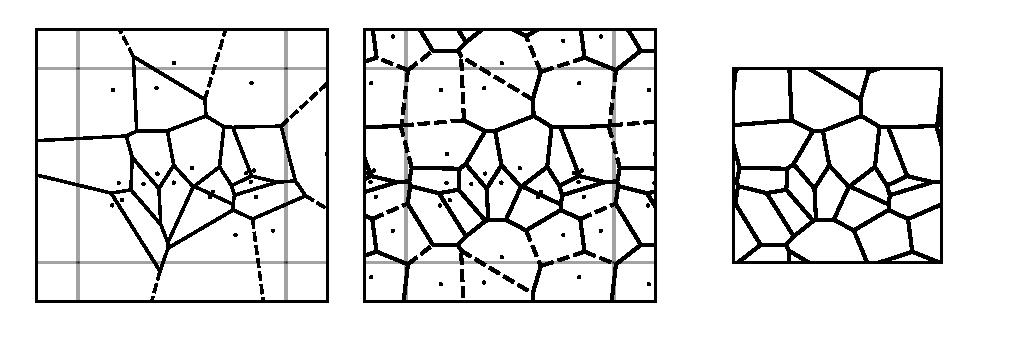
\includegraphics[width=1\textwidth,height=\textheight]{figure_code/amk_chapter/lattice_construction_animated/lattice_construction_animated}
\caption[{Lattice Construction}]{(Left) Lattice construction begins with the Voronoi partition of the plane with respect to a set of seed points (black points) sampled uniformly from \(\mathbb{R}^2\). (Center) However, we want the Voronoi partition of the torus, so we tile the seed points into a three by three grid. The boundaries of each tile are shown in light grey. (Right) Finally, we identify edges corresponding to each other across the boundaries to produce a graph on the torus. An edge colouring is shown here to help the reader identify corresponding edges. \href{http://thomashodson.com/assets/thesis/figure_code/amk_chapter/lattice_construction_animated/lattice_construction_animated.gif}{ Animated version online.}}
\label{fig:lattice_construction_animated}
\end{figure}
}

\hypertarget{graph-representation}{%
\subsection{Graph Representation}\label{graph-representation}}

Three keys pieces of information allow us to represent amorphous lattices.

Most of the graph connectivity is encoded by an ordered list of edges \((i,j)\). These are ordered to represent both directed and undirected graphs. This is useful for defining the sign of bond operators \(u_{ij} = - u_{ji}\).

Information about the embedding of the lattice onto the torus is encoded into a point on the unit square associated with each vertex. The torus is unwrapped onto the square by defining an arbitrary pair of cuts along the major and minor axes. For simplicity, we take these axes to be the lines \(x = 0\) and \(y = 0\). We can wrap the unit square back up into a torus by identifying the lines \(x = 0\) with \(x = 1\) and \(y = 0\) with \(y = 1\).

Finally, we need to encode the topology of the graph. This is necessary because, if we are simply given an edge \((i, j)\) we do not know how the edge gets from vertex i to vertex j. One method would be taking the shortest path, but it could also `go the long way around' by crossing one of the cuts. To encode this information, we store an additional vector \(\vec{r}\) associated with each edge. \(r_i^x = 0\) means that edge i does not cross the x. \(r_i^x = +1\) (\(-1\)) means it crossed the cut in a positive (negative) sense.

This description of the lattice has a very nice relationship to Bloch's theorem. Applying Bloch's theorem to a periodic lattice essentially means wrappping the unit cell onto a torus. Variations that happen at longer length scales than the size of the unit cell are captured by the crystal momentum. The crystal momentum inserts a phase factor \(e^{i \vec{q}\cdot\vec{r}}\) onto bonds that cross to adjacent unit cells. The vector \(\vec{r}\) is exactly what we use to encode the topology of our lattices.

\hypertarget{fig:bloch}{%
\begin{figure}
\centering
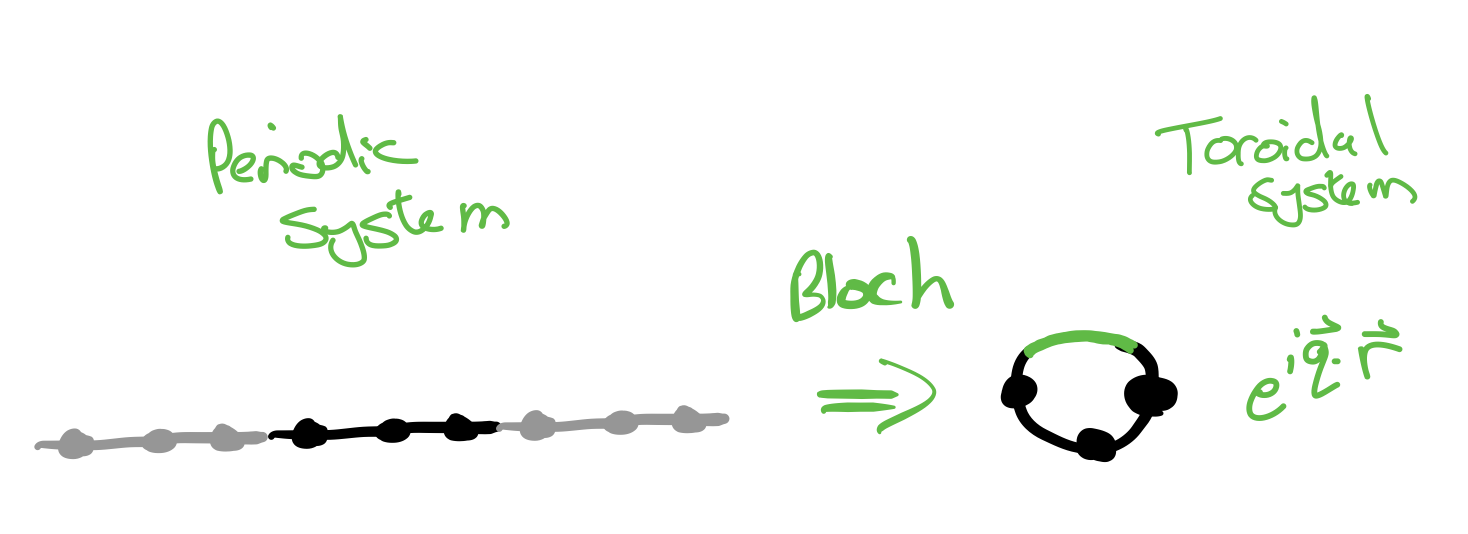
\includegraphics[width=1\textwidth,height=\textheight]{figure_code/amk_chapter/methods/bloch.png}
\caption[{Bloch's Theorem and the Torus}]{Bloch's theorem can be thought of as transforming from a periodic Hamiltonian on the place to the unit cell defined an torus. In addition we get some phase factors \(e^{i\vec{k}\cdot\vec{r}}\) associated with bonds that cross unit cells that depend on the sense in which they do so \(\vec{r} = (\pm1, \pm1)\). Representing graphs on the torus turns out to require a similar idea, we unwrap the torus to one unit cell and keep track of which bonds cross the cell boundaries.}
\label{fig:bloch}
\end{figure}
}

\hypertarget{colouring-the-bonds}{%
\subsection{Colouring the Bonds}\label{colouring-the-bonds}}

The Kitaev Model requires that each edge in the lattice be assigned a label \(x\), \(y\) or \(z\), such that each vertex has exactly one edge of each type connected to it. Let \(\Delta\) be the maximum degree of a graph which, in our case, is 3. If \(\Delta > 3\), it is obviously not possible to three-colour the edges. However, the general theory of when this is and is not possible for graphs with \(\Delta \leq 3\) is more subtle.

In the graph theory literature, graphs where all vertices have degree three are commonly called cubic graphs. There is no term for graphs with maximum degree three. Planar graphs are graphs which can be embedded onto the plane without any edges crossing. Bridgeless graphs do not contain any edges that, when removed, would partition the graph into disconnected components.

This problem must be distinguished from that considered by the famous four-colour theorem~\autocite{appelEveryPlanarMap1989}. The 4-colour theorem is concerned with assigning colours to the \textbf{vertices} of a graph, such that no vertices that share an edge have the same colour. Here we are concerned with an edge colouring.

The four-colour theorem applies to planar graphs, those that can be embedded onto the plane without any edges crossing. Here we are concerned with Toroidal graphs, which can be embedded onto the torus without any edges crossing. In fact, toroidal graphs require up to seven colours~\autocite{heawoodMapColouringTheorems}. The complete graph \(K_7\) is a good example of a toroidal graph that requires seven colours.

\(\Delta + 1\) colours are enough to edge-colour any graph. An \(\mathcal{O}(mn)\) algorithm exists to do it for a graph with \(m\) edges and \(n\) vertices~\autocite{gEstimateChromaticClass1964}. Restricting ourselves to graphs with \(\Delta = 3\) like ours, those can be four-edge-coloured in linear time~\autocite{skulrattanakulchai4edgecoloringGraphsMaximum2002}.

However, three-edge-colouring them is more difficult. Cubic, planar, bridgeless graphs can be three-edge-coloured if and only if they can be four-face-coloured~\autocite{tait1880remarks}. An \(\mathcal{O}(n^2)\) algorithm exists here~\autocite{robertson1996efficiently}. However, it is not clear whether this extends to cubic, \textbf{toroidal} bridgeless graphs.

\hypertarget{fig:multiple_colourings}{%
\begin{figure}
\centering
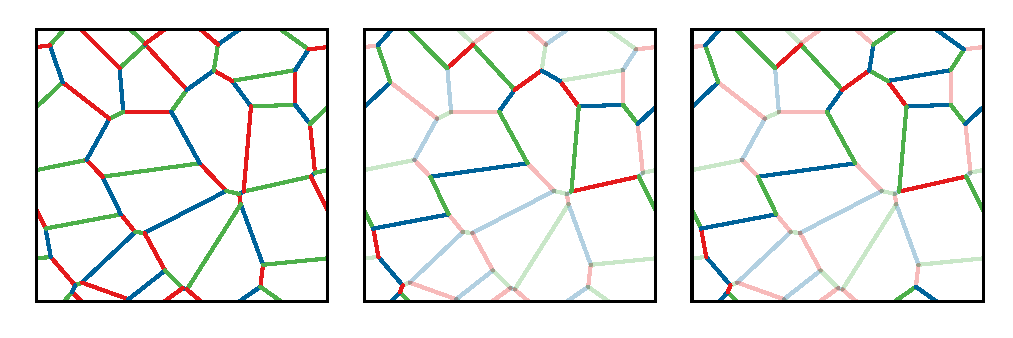
\includegraphics[width=1\textwidth,height=\textheight]{figure_code/amk_chapter/multiple_colourings/multiple_colourings}
\caption[{Colourings of an Amorphous Lattice}]{Three different valid 3-edge-colourings of amorphous lattices. Colors that differ from the leftmost panel are highlighted.}
\label{fig:multiple_colourings}
\end{figure}
}

\hypertarget{four-colourings-and-three-colourings}{%
\subsubsection{Four-colourings and three-colourings}\label{four-colourings-and-three-colourings}}

\textbf{add diagram of this}

A four-face-colouring can be converted into a three-edge-colouring quite easily: 1. Assume the faces of G can be four-coloured with labels (0,1,2,3) 2. Label each edge of G according to \(i + j \;\textrm{mod}\; 3\) where i and j are the labels of the face adjacent to that edge. For each edge label there are two face label pairs that do not share any face labels. i,e the edge label \(0\) can come about either from faces \(0 + 3\) or \(1 + 2\).

Explicitly, the mapping from face labels to edge labels is:

\[\begin{aligned}
0 + 3 \;\mathrm{or}\; 1 + 2 &= 0 \;\mathrm{mod}\; 3\\ 
0 + 1 \;\mathrm{or}\; 2 + 3 &= 1 \;\mathrm{mod}\; 3\\
0 + 2 \;\mathrm{or}\;1 + 3 &= 2 \;\mathrm{mod}\; 3\\
\end{aligned}
\]

\begin{enumerate}
\def\labelenumi{\arabic{enumi}.}
\setcounter{enumi}{2}
\item
  In a cubic planar G, a vertex v in G is always part of three faces and the colours of those faces determine the colours of the edges that connect to v. The three faces must take three distinct colours from the set \(\{0,1,2,3\}\).
\item
  From there, one can easily be convinced that those three distinct face colours can never produce repeated edge colours according to the \(i+j \;\mathrm{mod}\; 3\) rule.
\end{enumerate}

This implies that all cubic planar graphs are three-edge-colourable. This does not apply to toroidal graphs. We have not yet generated a Voronoi lattices on the torus that is not three-edge-colourable. This suggests that Voronoi lattices may have additional structures that make them three-edge-colourable. Intuitively, it seems that the kinds of toroidal graphs that cannot be three-edge-coloured could never be generated by a Voronoi partition with more than a few seed points.

\hypertarget{finding-lattice-colourings-with-minisat}{%
\subsubsection{Finding Lattice colourings with miniSAT}\label{finding-lattice-colourings-with-minisat}}

Some issues are harder in theory than in practice. Three-edge-colouring cubic toroidal graphs appears to be one of those things.

To find colourings, we use a Boolean Satisfiability Solver or SAT solver. A SAT problem is a set of statements about some number of boolean variables , such as ``\(x_1\) or not \(x_3\) is true'', and looks for an assignment \(x_i \in {0,1}\) that satisfies all the statements~\autocite{Karp1972}.

General purpose, high performance programs for solving SAT problems have been an area of active research for decades~\autocite{alounehComprehensiveStudyAnalysis2019}. Such programs are useful because, by the Cook-Levin theorem, any NP problem can be encoded in polynomial time as an instance of a SAT problem . This property is what makes SAT one of the subset of NP problems called NP-Complete~\autocite{cookComplexityTheoremprovingProcedures1971,levin1973universal}.

Thus, it is a relatively standard technique in the computer science community to solve NP problems by first transforming them to SAT instances and then using an off the shelf SAT solver. The output of this can then be mapped back to the original problem domain.

NP problems can be loosely considered as those which do not have a special structure than can be exploited to compute their solution in polynomial time. Our three-edge-colouring problem is likely not in NP. However, since we do not know what special structure it might have that could be used to speed up its solution, using a SAT solver appears to be a reasonable first method to try. As will be discussed later, this turned out to work well enough and looking for a better solution was not necessary.

We use a solver called \passthrough{\lstinline!MiniSAT!}~\autocite{imms-sat18}. Like most modern SAT solvers, \passthrough{\lstinline!MiniSAT!} requires the input problem to be specified in Conjunctive Normal Form (CNF). CNF requires that the constraints be encoded as a set of \emph{clauses} of the form \[x_1 \;\textrm{or}\; -x_3 \;\textrm{or}\; x_5\] that contain logical ORs of some subset of the variables where any of the variables may also be logically NOT'd, which we represent by negation here.

A solution of the problem is one that makes all the clauses simultaneously true.

We encode the edge colouring problem by assigning \(3B\) boolean variables to each of the \(B\) edges of the graph, \(x_{i\alpha}\) where \(x_{i\alpha} = 1\) indicates that edge \(i\) has colour \(\alpha\).

For edge colouring graphs we need two types of constraints: 1. Each edge is exactly one colour. 2. No neighbouring edges are the same colour.

The first constraint is a product of doing this mapping to boolean variables. The solver does not know anything about the structure of the problem unless it is encoded into the variables.

Let's say we have three variables that correspond to particular edge being red \(r\), green \(g\) or blue \(b\).

To require that exactly one of the variables be true, we can enforce that no pair of variables be true: \passthrough{\lstinline!-(r and b) -(r and g) -(b and g)!}

However, these clauses are not in CNF form. Therefore, we also have to use the fact that \passthrough{\lstinline!-(a and b) = (-a OR -b)!}. To enforce that at least one of these is true we simply OR them all together \passthrough{\lstinline!(r or b or g)!}

To encode the fact that no adjacent edges can have the same colour, we emit a clause that, for each pair of adjacent edges, they cannot be both red, both green or both blue.

We get a solution or set of solutions from the solver, which we can map back to a labelling of the edges. \cref{fig:multiple_colourings} shows some examples.

The solution presented here works well enough for our purposes. It does not take up a substantial fraction of the overall computation time, see +fig:times but other approaches could likely work.

When translating problems to CNF form, there is often some flexibility. For instance, we used three boolean variables to encode the colour of each edge and, then, additional constraints to require that only one of these variables be true. An alternative method which we did not try would be to encode the label of each edge using two variables, yielding four states per edge, and then add a constraint that one of the states, say (true, true) is disallowed. This would, however, have added some complexity to the encoding of the constraint that no adjacent edges can have the same colour.

The popular \emph{Networkx} Python library uses a greedy graph colouring algorithm. It simply iterates over the vertices/edges/faces of a graph and assigns them a colour that is not already disallowed. This does not work for our purposes because it is not designed to look for a particular n-colouring. However, it does include the option of using a heuristic function that determine the order in which vertices will be coloured~\autocite{kosowski2004classical,matulaSmallestlastOrderingClustering1983}. Perhaps

\hypertarget{fig:times}{%
\begin{figure}
\centering
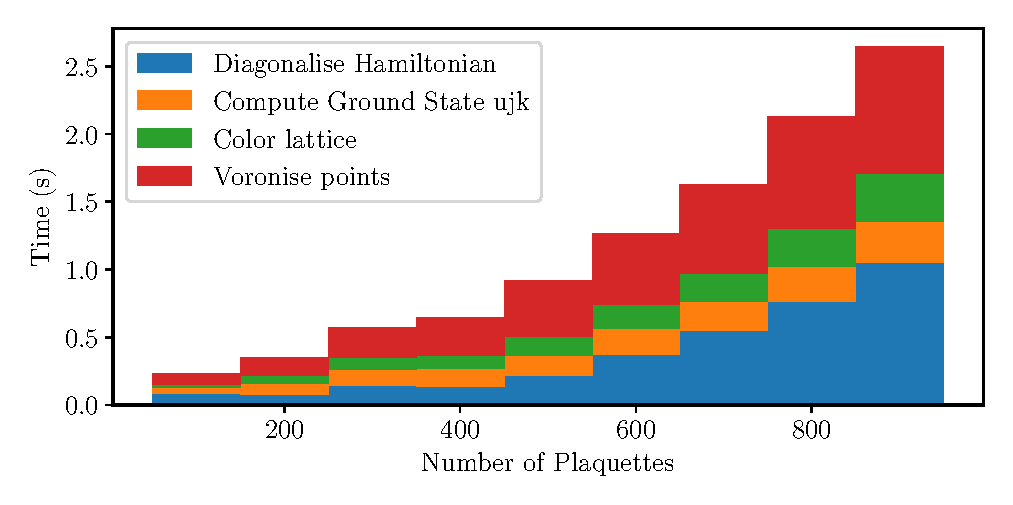
\includegraphics[width=1\textwidth,height=\textheight]{figure_code/amk_chapter/methods/times/times}
\caption[{Computation Time Spent on Different Procedures.}]{The proportion of computation time taken up by the four longest running steps when generating a lattice. For larger systems, the time taken to perform the diagonalisation dominates.}
\label{fig:times}
\end{figure}
}

\hypertarget{does-it-matter-which-colouring-we-choose}{%
\subsubsection{Does it matter which colouring we choose?}\label{does-it-matter-which-colouring-we-choose}}

In the isotropic case \(J^\alpha = 1\), it is easy to show that choosing a particular valid colouring cannot make a difference. As the choice of how we define the four Majoranas at a site is arbitrary, we can define a local operator that transforms the colouring of any particular site to another permutation. The operators commute with the Hamiltonian and, by composing such operators, we can transform the Hamiltonian generated by one colouring into that generated by another.

We cannot do this in the anisotropic case. It remains an open question whether particular physical properties could arise by engineering the colouring in this phase though we expect them to exhibit a self averaging behaviour.

\hypertarget{mapping-between-flux-sectors-and-bond-sectors}{%
\subsection{Mapping between flux sectors and bond sectors}\label{mapping-between-flux-sectors-and-bond-sectors}}

Constructing the Majorana representation of the model requires the particular bond configuration \(u_{jk} = \pm 1\). However, the large number of gauge symmetries of the bond sector makes it unwieldy to work with. Therefore, we need a way to quickly map between bond sectors and flux sectors.

Going from the bond sector to flux sector is easy. We can compute it directly by taking the product of \(i u_{jk}\) around each plaquette \[ \phi_i = \prod_{(j,k) \; \in \; \partial \phi_i} i u_{jk}\]

Going from flux sector to bond sector requires more thought. The algorithm we use is this:

\begin{enumerate}
\def\labelenumi{\arabic{enumi}.}
\item
  Fix the gauge by choosing some arbitrary \(u_{jk}\) configuration. In practice, we use \(u_{jk} = +1\). This chooses an arbitrary one of the four topological sectors.
\item
  Compute the current flux configuration and how it differs from the target one. We refer to a plaquette that differs from the target as a ``defect''.
\item
  Find any adjacent pairs of defects and flip the \(u_jk\) between them. This leaves a set of isolated defects.
\item
  Pair the defects up using a greedy algorithm.
\item
  Compute paths along the dual lattice between each pair of plaquettes. Flipping the corresponding set of bonds transports one flux to the other and annihilates them.
\end{enumerate}

\hypertarget{fig:flux_finding}{%
\begin{figure}
\centering
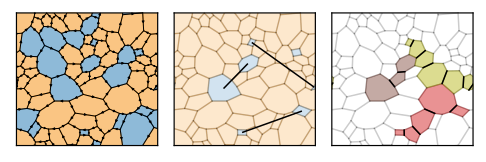
\includegraphics[width=1\textwidth,height=\textheight]{figure_code/amk_chapter/flux_finding/flux_finding}
\caption[{Finding Bond Sectors from Flux Sectors}]{(Left) The ground state flux sector and bond sector for an amorphous lattice. Bond arrows indicate the direction in which \(u_{jk} = +1\). Plaquettes are coloured blue when \(\hat{\phi}_i = -1\) (\(-i\)) for even/odd plaquettes and orange when \(\hat{\phi}_i = +1\) (\(+i\)) for even/odd plaquettes. (Centre) To transform this to the target flux sector (all \(+1\)/\(+i\)), we first flip any \(u_{jk}\) that are between two fluxes. This leaves a set of isolated fluxes that must be annihilated. Then, these are paired up as indicated by the black lines. (Right) A* search is used to find paths (coloured plaquettes) on the dual lattice between each pair of fluxes and the corresponding \(u_{jk}\) (shown in black) are flipped. One flux will remain because the starting and target flux sectors differed by an odd number of fluxes.}
\label{fig:flux_finding}
\end{figure}
}

\hypertarget{chern-markers}{%
\subsection{Chern Markers}\label{chern-markers}}

We know that the standard Kitaev model supports both Abelian and non-Abelian phases. Therefore, how can we assess whether this is also the case for the amorphous Kitaev model?

We have already discussed the fact that topology and anyonic statistics are intimately linked. This will help here. The Chern number is a quantity that measures the topological characteristics of a material.

The original definition of the Chern number relies on the model having translation symmetry. This leads to the development of \emph{local markers}. These are operators that generalise the notion of the Chern number to an observable over some region smaller than the entire system.

\textbf{Expand on definition here}

\textbf{Discuss link between Chern number and Anyonic Statistics}
